9. По теореме Виета $x_1+x_2=8,\ x_1x_2=q.$ Тогда $x_1^2+x_2^2=(x_1+x_2)^2-2x_1x_2=64-2q=34,\ q=15.$ Параболу $x^2-8x+15$ построим по трём точкам $(3;0),\ (5;0),\ (4;-1).$
$$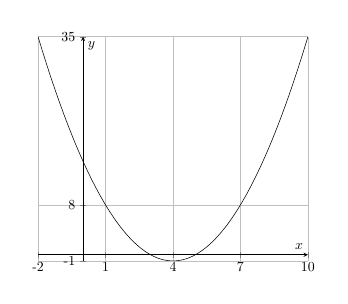
\begin{tikzpicture}[scale=0.5]
\begin{axis}[
    axis lines = middle,
    grid=major,
    legend pos={south west},
    xlabel = {$x$},
    ylabel = {$y$},
    %ymin=-80,
    %ymax=250,
    xtick={-2, 1, 4, 7, 10},
    xticklabels={-2, 1, 4, 7, 10},
    ytick={-1,8,35},
    yticklabels={-1,8,35}             ]
	\addplot[domain=-2:10, samples=100, color=black] {x*x-8*x+15};
%\addplot[domain=-3.1:2.5, samples=100, color=red] {70*abs(1-2*abs(abs(x)-2))-10*x^2+10*x-70};
	%\addlegendentry{$\text{Рис. 1}$};
\end{axis}
\end{tikzpicture}$$
